\documentclass[12pt]{article}

%%%%%%%%%%%%%%%%%%%%%%%%%%%%%%%%%%%%%%%%%%%%%%%%%%%%%%%%%%%%%%%%%%%%%
%% Place any additional packages needed here.  Only include packages
%% which are essential, to avoid problems later.
%%%%%%%%%%%%%%%%%%%%%%%%%%%%%%%%%%%%%%%%%%%%%%%%%%%%%%%%%%%%%%%%%%%%%
\usepackage{hyperref}
\usepackage[margin=1in]{geometry}
\usepackage{mathptmx}
\usepackage{fancyhdr}
\usepackage{lastpage}

\setcounter{secnumdepth}{0}% % Turns off numbering for sections
\pagestyle{fancy}
\rhead{ Singh, Gurpreet.  Bartlett, Paul. }
\lhead{\thepage\ of \pageref{LastPage}}

\usepackage{chemformula} % Formula subscripts using \ch{}
\usepackage[T1]{fontenc} % Use modern font encodings
\usepackage[utf8]{inputenc} % Required for inputting international characters
\usepackage[T1]{fontenc} % Output font encoding for international characters

\hypersetup{
    pdftitle={Faulty: Fault Localization as a Service},    % title
    pdfauthor={},     % author
    pdfcreator={},   % creator of the document
}

\providecommand{\tightlist}{%
  \setlength{\itemsep}{0pt}\setlength{\parskip}{0pt}}

%%%%%%%%%%%%%%%%%%%%%%%%%%%%%%%%%%%%%%%%%%%%%%%%%%%%%%%%%%%%%%%%%%%%%
%% If issues arise when submitting your manuscript, you may want to
%% un-comment the next line.  This provides information on the
%% version of every file you have used.
%%%%%%%%%%%%%%%%%%%%%%%%%%%%%%%%%%%%%%%%%%%%%%%%%%%%%%%%%%%%%%%%%%%%%
%%\listfiles

%%%%%%%%%%%%%%%%%%%%%%%%%%%%%%%%%%%%%%%%%%%%%%%%%%%%%%%%%%%%%%%%%%%%%
%% Place any additional macros here.  Please use \newcommand* where
%% possible, and avoid layout-changing macros (which are not used
%% when typesetting).
%%%%%%%%%%%%%%%%%%%%%%%%%%%%%%%%%%%%%%%%%%%%%%%%%%%%%%%%%%%%%%%%%%%%%

\begin{document}

%----------------------------------------------------------------------------------------
%	TITLE PAGE
%----------------------------------------------------------------------------------------

\begin{titlepage} % Suppresses displaying the page number on the title page and the subsequent page counts as page 1
	\newcommand{\HRule}{\rule{\linewidth}{0.5mm}} % Defines a new command for horizontal lines, change thickness here
	
	\center % Centre everything on the page
	
	%------------------------------------------------
	%	Headings
	%------------------------------------------------
	
	\textsc{\LARGE University of Western Ontario}\\[0.8cm] % Main heading such as the name of your university/college

	\textsc{\Large Department of Computer Science}\\[1.5cm] % Major heading such as course name
	
	\textsc{\large CS4470Y: Software Maintenance and Configuration}\\[0.8cm] % Major heading such as course name
	
	\textsc{\large Final Project Report}\\[0.8cm] % Minor heading such as course title
	
	%------------------------------------------------
	%	Title
	%------------------------------------------------
	
	\HRule\\[0.4cm]
	
	{\huge\bfseries Faulty: Fault Localization as a Service}\\[0.4cm] % Title of your document
	
	\HRule\\[1.5cm]
	
	%------------------------------------------------
	%	Author(s)
	%------------------------------------------------
	
	\begin{minipage}{0.4\textwidth}
		\begin{flushleft}
			\large
			\textit{Author}\\
            			Gurpreet \textsc{Singh} \\             			Paul \textsc{Bartlett} \\ 		\end{flushleft}
	\end{minipage}
	~
	\begin{minipage}{0.4\textwidth}
		\begin{flushright}
            			    \large
			    \textit{Supervisor}\\
                                    Kostas \textsc{Kontogiannis}\\[0.5cm]
                            
                            \large
                \textit{Instructor}\\
                                    Nazim \textsc{Madhavji}\\
                            		\end{flushright}
	\end{minipage}
	
	% If you don't want a supervisor, uncomment the two lines below and comment the code above
	%{\large\textit{Author}}\\
	%John \textsc{Smith} % Your name

	%------------------------------------------------
	%	Date
	%------------------------------------------------

	\vfill\vfill % Position the date 3/4 down the remaining page
	
	{\large\today} % Date, change the \today to a set date if you want to be precise
	
	%------------------------------------------------
	%	Logo
	%------------------------------------------------
	
    	\vfill\vfill
	
\includegraphics[width=0.2\textwidth]{../images/uwo.jpg}\\[1cm] % Include a department/university logo - this will require the graphicx package
    	 
	%----------------------------------------------------------------------------------------
	
	\vfill % Push the date up 1/4 of the remaining page
	
\end{titlepage}

\begin{abstract} 
{\bf Aiming to reduce debugging time by making fault localization software
available to the masses via a software as a service solution} Most developers run into issues with finding the root cause of a bug
report. We begin with a distributed system of scripts that use code and
bug reports to find that root cause and we make it into an accessible
service for developers of all skill levels. We will be making use of a
GitHub workflow using a publisher/consumer model to fetch bugs and
provide analysis on them. Using a web UI for the continuous integration
tool will allow developers to easily adopt the tool into their projects.
Bringing the complex algorithms discovered in previous research to the
masses will greatly benefit large projects by reducing debugging time
and development resources \end{abstract} 

\section{Introduction}\label{introduction}

\subsubsection{Problem description}\label{problem-description}

Most professional developers and software engineers have run into a
situation where they are presented with a bug, issue, or ticket and do
not know where to begin looking for the cause of the problem. This
usually leads the developer into a long series of bruteforce debugging
where they explore all possible paths leading up to the symptoms hoping
they will run into something suspicious.

In an attempt to reduce this mindless guessing and time wasted for the
developer, the research of fault localization is used to
programmatically understand where the error could be coming from. The
project we are working with is capable of creating a list of files that
are most likely to have the bug within them.

\subsubsection{Focus}\label{focus}

Our focus will be to take that project and streamline the process so it
is easier for an average developer to pickup and plug into their project
to help their workflow. We will be creating a Software as a
Service(SaaS) using the concept of the BugLocalization project that
Professor Kontogainnis has organized in the past.

\subsubsection{Key results}\label{key-results}

We were able to significantly improve the existing codebases and reduce
a large amount of complexity from the processing. This allowed us to
easily plug the code into an API that we created. The API issues from a
Github repository and then initiates a modified version of the
BugLocalization process.

\subsubsection{Significance}\label{significance}

This work is very significant as it has the opportunity to be the first
easily pluggable fault localization software that can be used without
extensive resources. We hope in the future this service would be used as
commonly as other CI tools like Travis.

\subsubsection{Report Structure}\label{report-structure}

The report will first cover terms needed to understand the report, then
some background information about the algorithm and process used inside
BugLocalization and finally the objectives, strategy and results of our
development

\section{Concepts, Terms, Definitions,
Equations}\label{concepts-terms-definitions-equations}

\subsubsection{RSF}\label{rsf}

An RSF is a map of relationships betweens tokens within a codebase,
where a token is a keyword in the codebase such as a method. It is
generated using preprocessing scripts, and the result allows us to
verify tokens inside of bug reports.

\subsubsection{Bug Report}\label{bug-report}

A database entry for each bug report used for the analysis. Each bug
report contains a String field containing what a user wrote inside their
bug report.

\subsubsection{Token Expansion}\label{token-expansion}

Tokens extracted from the bug report are expanded to find other similar
tokens. Token expansion includes tokens that are referenced by the
original token set.

\subsubsection{Clique}\label{clique}

A collection of tokens that are referenced the most within the expanded
set of tokens

\subsubsection{Cluster}\label{cluster}

A group of relationships that are closely related to each other

\section{Background and Related Work}\label{background-and-related-work}

The main purpose of this project is to assist in locating faults so
developers can isolate errors quicker. There are three main categories
of fault localization: static-analysis/test-case based approach, machine
learning based approach, and a type based approach. The method that we
are expanding upon falls into the first category with an approach that
heavily relies on preforming static analysis on the code and bug texts.

This project was conceived from research that Professor Kontogainnis had
completed with past students regarding the task of determining faults in
a large codebase using only past bug reports. Past students had
experimented with multiple algorithms for processing large amounts of
bug reports in order to come up with an index of files that are most
likely to have a new bug within them.

The project operated in many phases. Each one containing one very
specific task. The first phase involved extracting bug reports from a
repository and parsing them through a reader into an object model that
allowed easier processing. The second phase handled pulling the source
code of the project and generating tokens. Tokens can be entities in the
codebase but for our specific use they are method names that are later
lifted up to filenames. A map of these tokens is created and then using
the results from phase 1 and 2, the next piece of software is ready to
make a connection between these two datasets. In phase 3 each of the
tokens extracted from the bug report are verified and expanded to
generate a set of tokens that include all relatives to each token. A
token's relative is defined as a token that makes a call to or from the
original token.

The first three phases mostly involved preprocessing different datasets
into a form that would be ideal for making a conclusion. At this point
we have a large set of entities that we suspect are vaguely related to
the bug report we want to process. Phase 4 is where we begin making
conclusions on the data. The software chooses between two algorithms for
determining the score that will indicate the faulty files. If the amount
of files associated with the bug are less than 15\% of the total system
files, we choose the simpler algorithm and find the score by determining
which files have the most outward connections to the codebase. If the
bug effects more than 15\% of total files, we generate clusters of
related entities using our relationship map produced in phase 2 and then
for each cluster we check how connected it is to the most important
files related to our bug. The cluster that is most connected has the
highest chance of containing the bug.(Krystalenia 2017, Ionna
Stavropoulou (2017))

The original system consisted of a collection of scripts written in
Java, Python and Shell. The scripts were fairly distributed and had very
little documentation. Most of the work was done in intermediate steps
and did not fit well together as a system because too much user
intervention was required between steps.

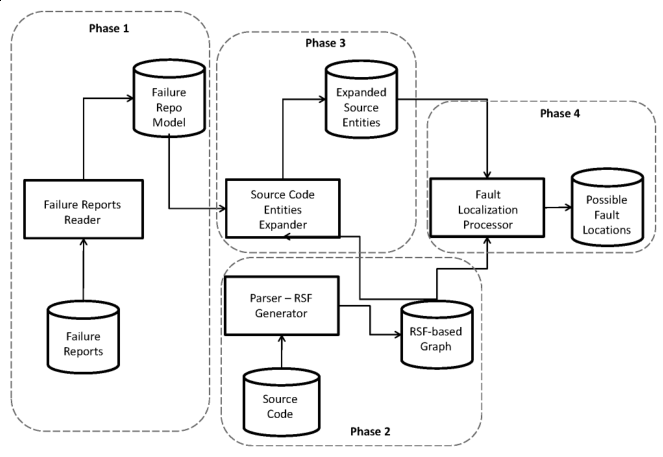
\includegraphics[width=500px]{../images/FaultPhases}

\section{Development Objectives}\label{development-objectives}

The focus will be to design and develop a system that is capable of
processing bug reports and extracting useful information about them, and
then using that information to provide the developers useful insight
into where the bug may be within a large code base. The goal is to
reduce the amount of time a developer will need to reach the correct bug
after initially reviewing the bug report.

The system will be developed in such a way that it is easily integrated
into a continuous delivery pipeline. The project can be divided into
three distinct components.

\subsubsection{Data Processing (O1)}\label{data-processing-o1}

In order for the entire system to work correctly the core essential data
processing and analysis has to be effective in detecting the errors.
Therefore, the first step is developing a system that can use NLP to
process all the bug reports associated with a project to come up with a
list of keywords and process the code base to determine a map of
relationships between function calls. This code has now been written and
is mostly within our project.

\subsubsection{User Interface (O2)}\label{user-interface-o2}

The next step in delivering the system to a real user, is developing a
front end where a user can input a repository for the system to begin
processing. Ideal operation of this tool would occur like other DevOps
pipeline tools such as travis-ci.org where a user can link a repository
they own and the tool can push it's results back into the bug report for
developers to see. There will not be too many interactions available on
the front end other than viewing the results of the system and picking
new repositories. This portion of the project is not yet completed.
Refer to deviations section to understand the reasoning for putting the
interface as the last priority.

\subsubsection{Runtime Processing (O3)}\label{runtime-processing-o3}

Since the front end will be making REST API calls to Github
repositories, and we need a way to persist processing while providing
consistent feedback to users, there needs to be a backend API service
allowing those operations to occur. Another task this portion will be
responsible for is handling the flow of information when a new bug
report appears. The backend will be responsible for detecting this,
starting a new processing task, and posting a ``Fault Report'' back into
the bug discussion. A substantial amount of work has been done on this
portion of the project. The backend is able to communicate with Github
and catch issues posted by users.

\section{System Requirements}\label{system-requirements}

\subsubsection{Section A : Data
Processing}\label{section-a-data-processing}

\begin{itemize}
\item
  \textbf{Feature 1:} Able to generate entity relationship rsf from
  codebase
\item
  FR 1: Pass code through cdif2rsf to generate rsf
\item
  FR 2: Clean up incorrect entity and relationships
\item
  FR 3: Store in accessible data storage for next step to use
\item
  \textbf{Feature 2:} Able to generate set of keywords from bug
  description
\item
  FR 1: Compare each token to codebase to find valid functions
\item
  FR 2: Expand initial token set by a factor of 3
\item
  FR 3: Use NLP to determine question context
\item
  \textbf{Feature 3:} Able to combine keywords and rsf into ranked
  outcomes
\item
  FR 1: Run LSI on each token and generate search space for each
\item
  FR 2: Expand the search space for each result in FR 1
\item
  FR 3: Find similarities between the initial token expansion and the
  final set of tokens
\item
  FR 4: Apply ranking equation from research paper to come up with final
  outcome
\end{itemize}

\subsubsection{Section B : Front-End User
Interface}\label{section-b-front-end-user-interface}

\begin{itemize}
\item
  \textbf{Feature 4:} User is able to scan and mark a new repository for
  processing
\item
  FR 1: Scan user's Github repos using Github's API
\item
  FR 2: Allow the user to select ones they wish to run processing on
\item
  FR 3: Remember which ones the user selected by storing on backend
\item
  \textbf{Feature 5:} User is able to view the results of a new bug
  report's processing
\item
  FR 1: Monitor output from backend endpoints showing new results for
  user's repos
\item
  FR 2: When a new bug report is created, and the processing finishes,
  show the output of that processing on a separate page
\item
  FR 3: Allow the user to rerun processing on a specific bug report by
  sending a request to backend
\item
  \textbf{Feature 6:} User is able to login using their Github
  credentials
\item
  FR 1: On first usage redirect user to Github's App authentication page
\item
  FR 2: Ask backend to associate bug reports and repositories with this
  user
\item
  FR 3: Redirect user to main UI
\end{itemize}

\subsubsection{Section C : Back-End Runtime
Processing}\label{section-c-back-end-runtime-processing}

\begin{itemize}
\item
  \textbf{Feature 7:} Support front-end operations
\item
  FR 1: Allow registration using Github Auth
\item
  FR 2: Allow retrieval of processing results for each bug report
\item
  FR 3: Support re-running processing on a specific bug report
\item
  FR 4: Create a API where the UI can fetch everything from
\item
  \textbf{Feature 8:} Manage the automation of Data Processing (F1, F2,
  and F3)
\item
  FR 1: Automate RSF generation when a new repository is linked
\item
  FR 2: Automate keyword generation when a new repository is linked
\item
  FR 3: Continuously improve and modify RSF and keywords as code/bugs
  change
\item
  \textbf{Feature 9:} Handle processing and evaluation when a new bug
  report comes in
\item
  FR 1: Monitor marked repositories for each registered user and trigger
  when new issue is filed
\item
  FR 2: Run through automated ranking algorithm
\item
  FR 3: Store result for later retrieval
\item
  FR 4: Be able to connect to a repository and fetch an issue when it is
  posted
\item
  \textbf{Feature 10:} Combine each element of data processing into the
  backend runtime
\item
  FR 1: Combine entity generation into token generation
\item
  FR 2: Combine FR1 with RSF processing all into one unit
\item
  FR 3: Move all functionality to an exposed part of the API
\item
  FR 4: Create all endpoints for data processing functionality
\end{itemize}

\section{Development Strategy}\label{development-strategy}

Since this project had many parts of it already implemented, just in
poor condition, we did not have many choices over what development tools
and languages to use. The majority of the project was written in Java,
with some separate Python scripts used for data manipulation at some of
the stages in the system.

Since we started the API from scratch, we had more choices on
technologies and tools in that section. The API was written in Kotlin
because it allowed us to have easy access to the Java code since it is
still a JVM language but also provide higher level functionality and
cleaner syntax to speed up development. The API is supported by MongoDB
for storing data from Github issues and the future UI.

Git and Github were used for collaboration between the two developers
and ngrok was used to host the services. Another tool that really helped
our development strategy was Robo3t as it allowed us to monitor the
MongoDB for incoming objects and see them in realtime.

All the datasets we used for our processing came from BugZilla as that
was the only platform supported by the preexisting preprocessing
scripts. The project repositories we accessed were amarok, konjueror,
k3b, and kopete.

\subsubsection{Technologies}\label{technologies}

\begin{itemize}
\tightlist
\item
  Kotlin
\item
  Python
\item
  Java
\item
  Javalin
\item
  MongoDB
\item
  Github Webhooks
\end{itemize}

\subsubsection{Tools}\label{tools}

\begin{itemize}
\tightlist
\item
  Intellij Idea
\item
  NeoVim
\item
  Robo3T
\item
  ngrok
\item
  Git
\item
  Github
\end{itemize}

\subsubsection{Datasets}\label{datasets}

\begin{itemize}
\tightlist
\item
  BugZilla bug reports
\item
  amarok repository
\item
  Konqueror repository
\item
  k3b repository
\item
  kopete repository
\end{itemize}

\section{Results}\label{results}

\subsubsection{BugLocalization Project}\label{buglocalization-project}

\begin{itemize}
\tightlist
\item
  Restructured and cleaned up codebase
\item
  Reduced very large codebase to 10 files
\item
  Documented and made more readable for easier integration
\item
  Cleaned up data flow to allow easier integration with API
\end{itemize}

The BugLocalization project has been completely revamped to work better
with the API design. A large amount of redundant code has been removed
and only the essential functionality exists. Everything has been
commented and documented for easier maintainability and modularity.

This project produces two types of output depending on the input and
which algorithm is chosen for processing the token scoring. Figures 4
and 5 show you examples of each type of output figure 4 shows the
results received when you run BugLocalization with a small bug and a
simple algorithm is chosen. Figure 5 shows the results when you run
BugLocalization with a large bug and make use of the complex ranking
algorithm.

\subsubsection{API}\label{api}

\begin{itemize}
\tightlist
\item
  Able to monitor a GitHub repo for events
\item
  Detect new issues and add into a Mongo database
\item
  Able to start and end deployments on Pull Requests
\end{itemize}

The API was started from scratch and has progressed into something that
can be relied on to fetch and process incoming bug reports and support a
future UI. Currently the API is able to catch incoming Github webhooks
and take repository information from the HTTP request. Using this
information and the object model of the repository it can create an
entry in the database to represent it. When new issues come in they are
added to the object model inside the database and when processing begins
it can read that model from the database.

The results produced by the API are visible inside the object model of
the database. This model populated with some dummy issues can be seen in
the Robo3t screenshot in figure 6

\newpage

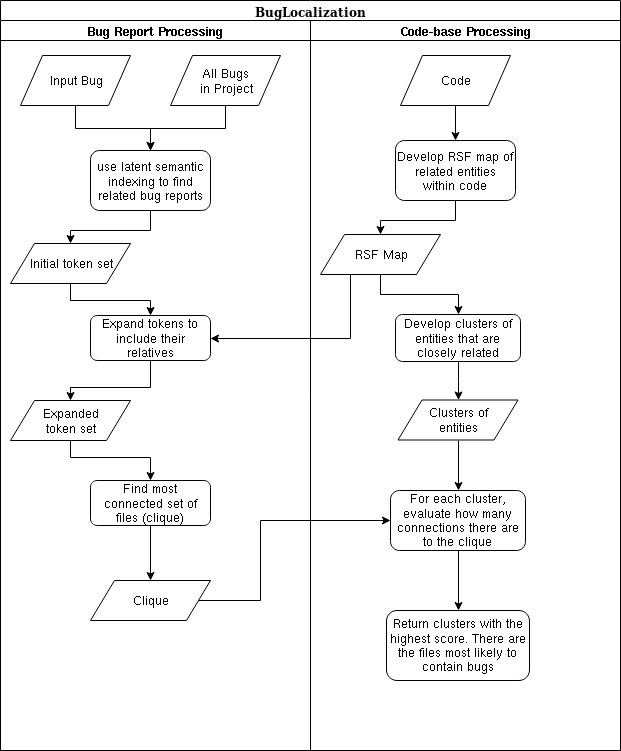
\includegraphics[width=500px]{../images/BugLocalizationFlow}
\emph{Figure 2}

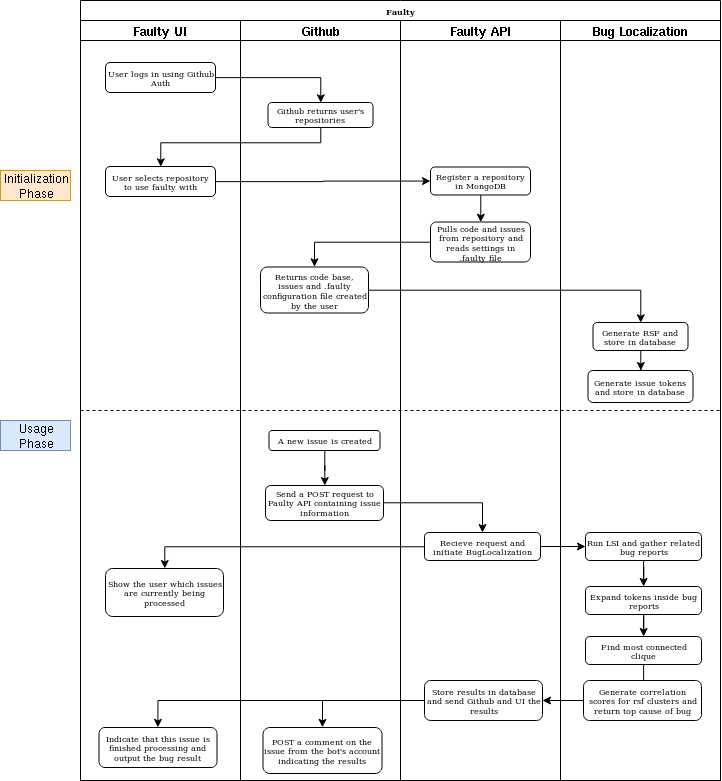
\includegraphics[width=500px]{../images/Flow} \emph{Figure 3}

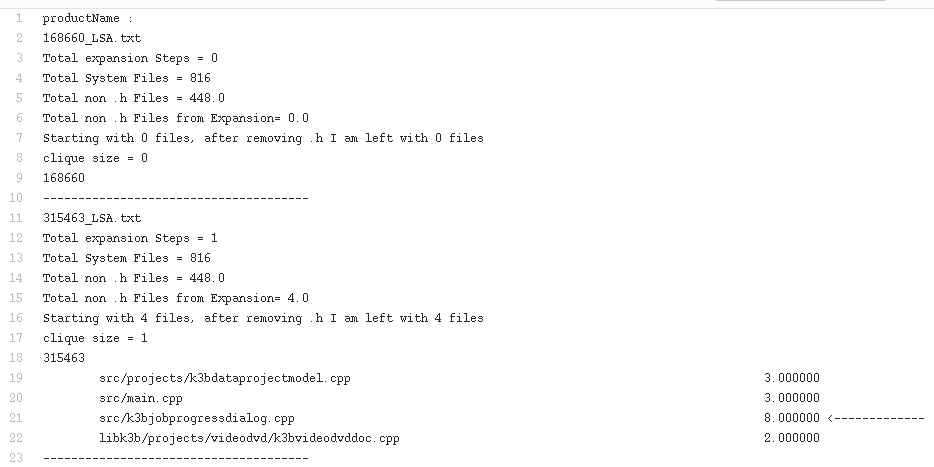
\includegraphics[width=500px]{../images/BLSimple} \emph{Figure 4}

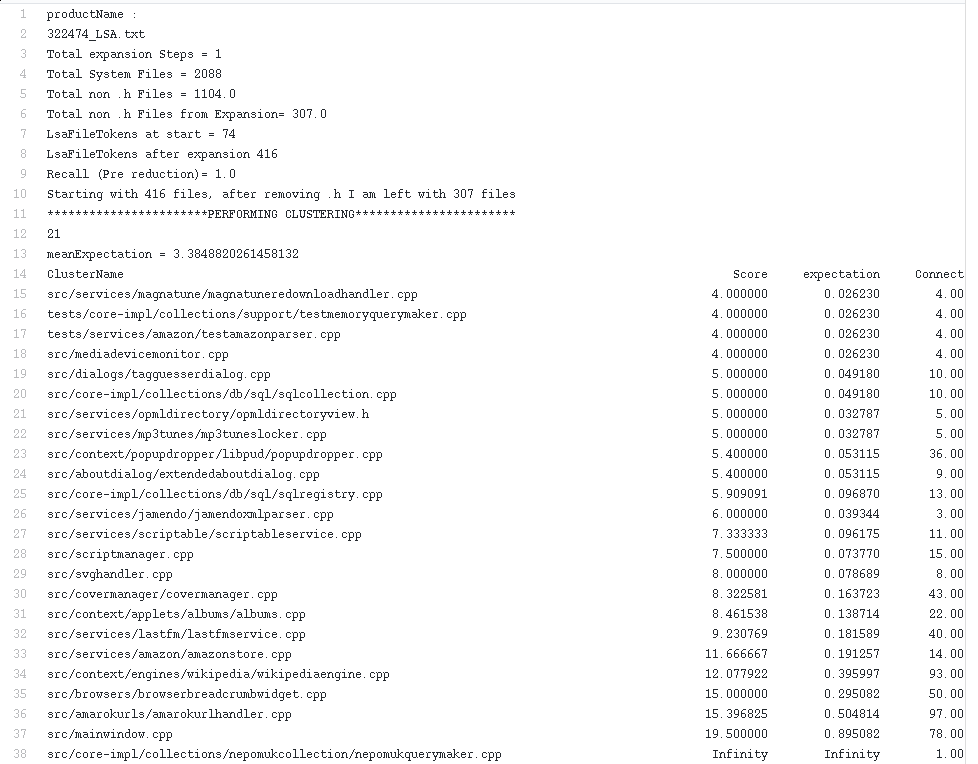
\includegraphics[width=500px]{../images/BLComplex} \emph{Figure 5}

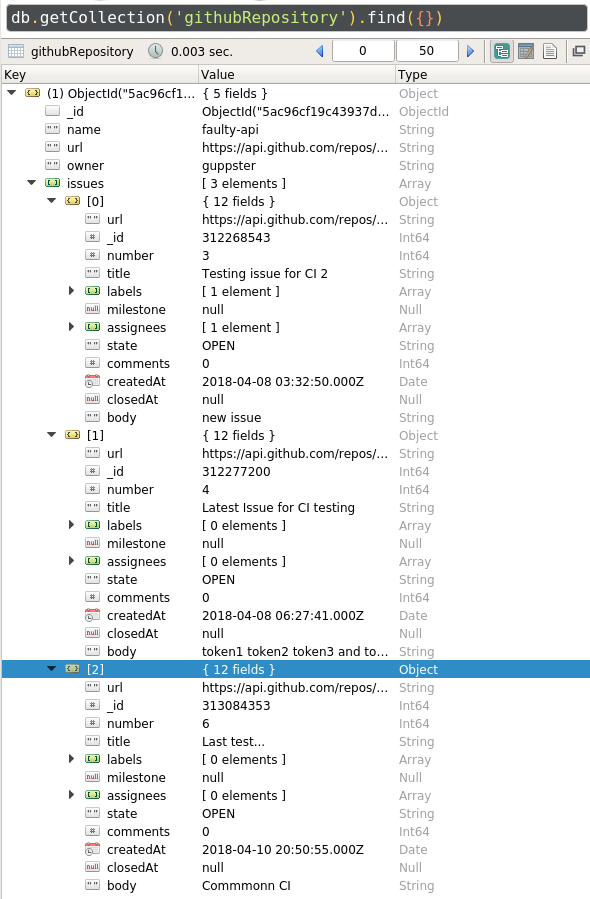
\includegraphics[width=400px]{../images/Robo3t} \emph{Figure 6}

\section{Discussion}\label{discussion}

\subsubsection{Threats to the validity of the
results}\label{threats-to-the-validity-of-the-results}

Due to the large amount of bug reports and the possibility of having
reports without enough details, the results are not guaranteed to find
where the fault occurs. The ranking used in the system is useful in
mitigating incorrect results, but does not ensure that any of the
results will be useful in determining the cause of fault in the
software. A lot of other methods used to minimize the threats to
validity were already implemented in the project, but it was mentioned
that using different algorithms would allow us to compare the accuracy
of different methods.

\subsubsection{Implications of the
results}\label{implications-of-the-results}

One of the original goals of this project was to implement another
algorithm for determining the cause of fault to then use to compare the
validity of the results for both algorithms. The validity of the results
is important for a system like this because of how flexible it is for
testing on software projects. The system would be language agnostic and
allow the user to be able to accurately detect specific points of faults
in software projects that use multiple languages. This is much more
useful than traditional tools used for detecting issues in software and
would be applicable to any project, where those that have large projects
and/or use multiple languages would benefit the most. This system would
save software engineers lots of time and effort wasted on debugging
issues with software systems that don't provide enough information about
where a fault in the program occurs.

\subsubsection{Limitations of the
results}\label{limitations-of-the-results}

The main limitation to this project is the complexity of being able to
detect a fault based on reports alone. When developing, users have many
methods of getting feedback through logs and error detection that are
not available to our system. The best way to remove this limitation
would be to get more details from failure reports, but unfortunately
there are not many alternatives that offer nearly as many reports as
BugZilla.

\section{Conclusions}\label{conclusions}

Unfortunately, for our project we had some communication problems for a
large portion of the year. We ended up getting a late start to the
project and had to re-purpose the project after the second milestone.
Due to our late start and a couple missing scripts, we did not have
access to all parts of the system needed to create a complete system and
did not have enough time to create a standalone service with a UI. The
implications of creating a complete system would mean that the computer
running the system would have to be powerful enough to process all parts
of the analysis within a reasonable amount of time in order to be of use
to the programmer. Based on our testing with the components we had, we
believe that this would be achievable if given access to the remaining
parts of the program. We were able to refactor the code and greatly
improve the structure and readability. The main method contained too
much of the logic of the system, so modularizing the code and adding
comments made it much easier to understand for others who will look at
the code.

Completing O2 added the ability to connect to GitHub using their API and
get issues from their tracker. Since the biggest change to the existing
system is the report data used, the main structure of the system remains
the same while allowing it to be used in another useful domain. Using
this system in GitHub allows developers to easily discover faults in
their applications. The system is set to be run whenever an issue was
added by a user and would notify the repo owner.

\section{Future Work and Lessons
Learnt}\label{future-work-and-lessons-learnt}

\subsubsection{Future work}\label{future-work}

For further development, we would want to develop software to process
issues incrementally into the BugLocalization. We would then integrate
the BugLocalization project as part of the API and utilize its full
power. Since we did not manage to complete O3, we would also want to
make a web UI similar to Travis to display results.

\subsubsection{Lessons learnt}\label{lessons-learnt}

We have learned from this project how important it is to develop
consistent communication plan with stakeholders. At many times during
this project, we went long periods of time without meeting to discuss
how our progress is going. This created some problems because we were
unsure of how to run the program initially and had to email a grad
student to get some of the missing files. Getting email responses took
longer than in person, so having more consistency to meet and discuss
problems in person would have been beneficial.

\newpage

\section*{References}\label{references}
\addcontentsline{toc}{section}{References}

\hypertarget{refs}{}
\hypertarget{ref-EMSE}{}
Ionna Stavropoulou, Kostas Kontogiannis, Marios Grigoriou. 2017. ``Case
Study on Which Relations to Use for Clustering-Based Software
Architecture Recovery.'' Springer.

\hypertarget{ref-Fault}{}
Krystalenia, Kostas Kontogiannis. 2017. ``Assisting Developers Towards
Fault Localization by Analyzing Failure Reports.'' CASCON. November.

\bibliography{}

%----------------------------------------------------------------------------------------

\end{document}
